\documentclass[12pt]{article}
\usepackage[top=1in, bottom=1in, left=1in, right=1in]{geometry}

\usepackage{setspace}
\onehalfspacing

\usepackage{amssymb}
%% The amsthm package provides extended theorem environments
\usepackage{amsthm}
\usepackage{epsfig}
\usepackage{times}
\renewcommand{\ttdefault}{cmtt}
\usepackage{amsmath}
\usepackage{graphicx} % for graphics files

% Draw figures yourself
\usepackage{tikz} 

% writing elements
\usepackage{mhchem}

% The float package HAS to load before hyperref
\usepackage{float} % for psuedocode formatting
\usepackage{xspace}

% from Denovo Methods Manual
\usepackage{mathrsfs}
\usepackage[mathcal]{euscript}
\usepackage{color}
\usepackage{array}

\usepackage[pdftex]{hyperref}
\usepackage[parfill]{parskip}

% math syntax
\newcommand{\nth}{n\ensuremath{^{\text{th}}} }
\newcommand{\ve}[1]{\ensuremath{\mathbf{#1}}}
\newcommand{\Macro}{\ensuremath{\Sigma}}
\newcommand{\rvec}{\ensuremath{\vec{r}}}
\newcommand{\vecr}{\ensuremath{\vec{r}}}
\newcommand{\omvec}{\ensuremath{\hat{\Omega}}}
\newcommand{\vOmega}{\ensuremath{\hat{\Omega}}}
\newcommand{\sigs}{\ensuremath{\Sigma_s(\rvec,E'\rightarrow E,\omvec'\rightarrow\omvec)}}
\newcommand{\el}{\ensuremath{\ell}}
\newcommand{\sigso}{\ensuremath{\Sigma_{s,0}}}
\newcommand{\sigsi}{\ensuremath{\Sigma_{s,1}}}
%---------------------------------------------------------------------------
%---------------------------------------------------------------------------
\begin{document}
\begin{center}
{\bf NE 250, F15\\
September 30, 2015 
}
\end{center}

Announcements:
\begin{itemize}
\item How I grade paragraphs
\item homework due friday; I'll also assign the next one that day
\end{itemize}

---------------------------------\\
Last time we were discussing the \underline{streaming term in curvilinear coordinates}.
Recall, $\vOmega \cdot \nabla$ is the derivative of angular flux along the direction of motion $\vOmega$. We will use the coordinate system (See Figure~\ref{fig:sph-coord}).
%
\begin{figure}[h!]
    \begin{center}
    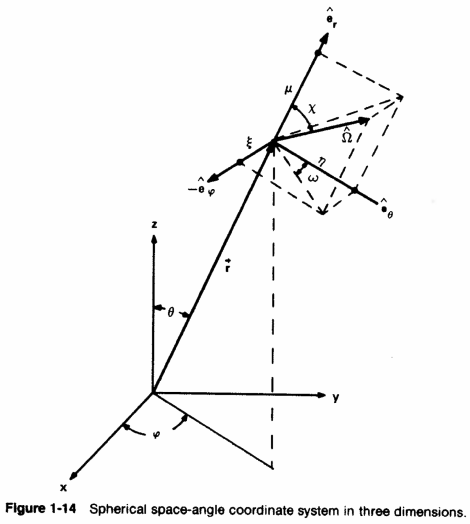
\includegraphics[keepaspectratio, width = 3.5 in]{../figs/spherical-coords}
    \end{center}    
    \label{fig:sph-coord} 
    \caption{Spherical: L\&M Chp.\ 1}
\end{figure}

In curvilinear geometry, neutrons ``migrate" across $\vOmega$ as they stream in straight lines. 
We can see this in spherical geometry (note, $dr$, $d\theta$, and $ds$ are assumed to be very small) and use that figure to understand our derivatives. Also recall sin = O/H, cos = A/H, and $\sin^2 + \cos^2 = 1$.
%
\begin{figure}[h!]
    \begin{center}
    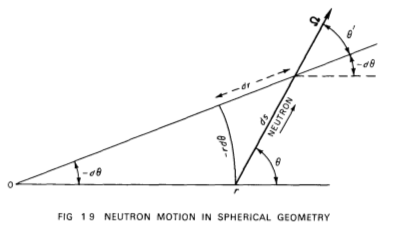
\includegraphics[keepaspectratio, width = 4.5 in]{../figs/n-motion-sph}
    \end{center}    
    \label{fig:sph-m} 
    \caption{Spherical: B\&G Chp.\ 1}
\end{figure}

\begin{align*}
\frac{d \psi}{ds} &= \frac{d \psi}{dr} \frac{dr}{ds} + \frac{d\psi}{d\mu} \frac{d\mu}{ds} \\
&\text{Look a the figure to define the terms}\\
\frac{dr}{ds} &= \cos(\theta) = \mu \\
%
\frac{d \mu}{ds} &= -\sin(\theta) \frac{d \theta}{ds} = -\sin(\theta) \biggl(\frac{-\sin(\theta)}{r} \biggr) = \biggl(\frac{1 - \mu^2}{r} \biggr) \\
%
\frac{d\psi}{ds} &= \mu \frac{\partial \psi}{\partial r} + \underbrace{\frac{(1 - \mu^2)}{r}\frac{\partial \psi}{\partial \mu}}_{\text{redistribution term}}
\end{align*}
%
We can extend all of that we get the ``conservation form" of the term (see B\&G 1.3b for derivation)
\[\frac{d\psi}{ds} = \frac{\mu}{r^2} \frac{\partial(r^2 \psi)}{\partial r} + \frac{1}{r} \frac{\partial}{\partial \mu}\bigl[(1 - \mu^2) \psi \bigr] \:. \]

I've included a table of the spherical conservative form terms as well as the coordinate system and conservative form for cylindrical coordinates in the notes.
%
\begin{figure}[h!] 
    \label{fig:sph-op}
    \begin{center}
    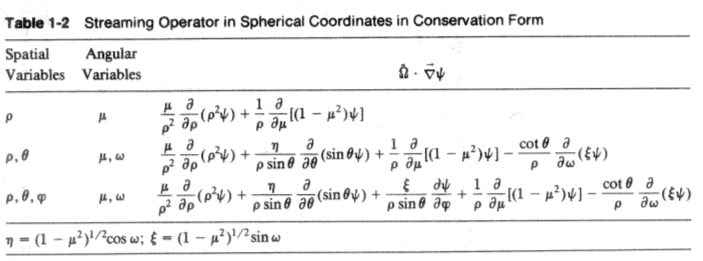
\includegraphics[keepaspectratio, width = 6 in]{../figs/spherical-operator}
    \end{center}    
\end{figure}

\begin{figure}[h!]
    \begin{center}
    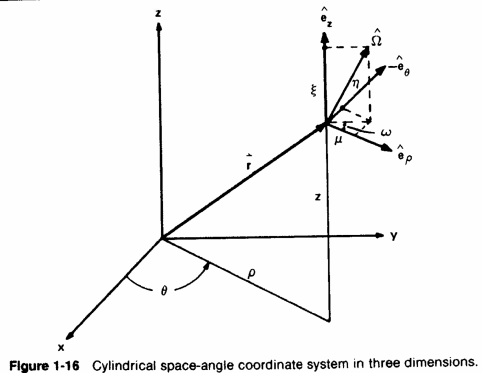
\includegraphics[keepaspectratio, width = 4 in]{../figs/cyl-coords}
    \end{center}    
    \label{fig:cyl-coord}
    \begin{center}
    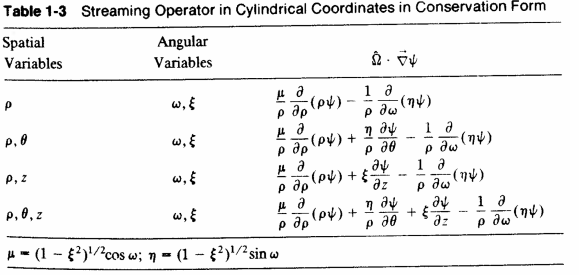
\includegraphics[keepaspectratio, width = 5 in]{../figs/cyl-operator}
    \end{center}    
    \caption{Cylindrical: L\&M Chp.\ 1}
\end{figure}

\clearpage
%------------------------------------------------------------
Back to \textbf{Eigenvalues and Criticality}

In the transport model (separation of variables):
\begin{align*}
\psi(\rvec, E, \vOmega, t) &= T(t) \Psi(\rvec, E, \vOmega) \\
T(t) &= \tau \exp(\alpha t) \quad \alpha \text{ depends on the evals of the ss transport operator} \\
\text{Eigenproblem: }L\Psi(\rvec, E, \vOmega) &= \frac{\alpha}{v}\Psi(\rvec, E, \vOmega)
\end{align*}
%
Homogeneous boundary conditions.\\
A non-trivial solution requires $(L - \frac{\alpha}{v})$ is singular. \\
That is, for $\Psi \neq 0 \rightarrow \: \alpha = v L$, which causes $L - \frac{\alpha}{v}$ to be zero, or non-invertible.

Linear operators: $L(a*x + b*y) = aL(x) + bL(y)$, where $a$ and $b$ and constants and $x$ and $y \: \in \: L$.\\
Examples are the derivative operator and integration. \\
A counter example is a quadratic:
\begin{align*}
L(z) &= z^2 \\
L(a(x) + b(y)) &= (ax + by)^2 = a^2 x^2 + axby + b^2 y^2 \\
& \neq \underbrace{a x^2}_{aL(x)} + \underbrace{b x^2}_{bL(x)}
\end{align*}
%
Our transport operator is linear, so each eval gives an emode, and the solution is a superposition of all emodes. \\
The collection of evals defines the spectrum of $L$.

Superposition of emodes for the general soln of the TE:
\begin{align*}
\psi(\rvec, E, \vOmega, t) &= \sum_{j} \tau_j \exp[\alpha_j t] \Psi_j(\rvec, E, \vOmega) \\
\psi(\rvec, E, \vOmega, 0) &= \sum_{j} \tau_j \Psi_j(\rvec, E, \vOmega) \quad \text{(known)}
\end{align*}

The fundamental emode corrsponds to $\max(Re(\alpha_j))$
\begin{itemize}
\item critical: $\max(Re(\alpha_j)) = 0$ for some $j$. All components but this one will attenuate. 
\item subcritical: $\max(Re(\alpha_j)) < 0 \: \forall j$.
\item supercritical: $\max(Re(\alpha_j)) > 0$ for some $j$, which gives growing eigenmode(s).
\end{itemize}
We denote the fundamental mode by $j=0$, $\alpha_0$. \\
This dominates the solution as $t \rightarrow \infty$:
\[\lim\limits_{t \to \infty} \psi(\rvec, E, \vOmega, t) = \Psi_0(\rvec, E, \vOmega)\]
and $\Psi_0$ must be real and positive.

\begin{itemize}
\item $\alpha_0 = 0$ is the criticality condition; gives a singular operator.
\item \textit{Given} a composition and geometry, $\alpha_j \rightarrow \psi$ for all time.
\item \textit{Determine} composition and geometry, $\alpha_0 = 0$ for criticality, $\alpha_j$ are evals.
\end{itemize}

\vspace*{1 em}
\underline{Existence of SS Soln to TE}
\[\frac{1}{v}\frac{\partial \psi}{\partial t} = L\psi + S = 0\]
in steady state (assumes $L$ and $S$ are time independent).

\begin{enumerate}
\item $\alpha_0 < 0$: $\psi$ decays in time; there is a non-zero $\psi$ that balances production and loss $\rightarrow$ a ss soln exists.
\item $\alpha_0 = 0$: if $S \neq 0$, then ss soln is unbounded \\
\hspace*{3.5 em}if $S=0$, then ss soln is $\Psi_0$.
\item $\alpha_0 > 0$: a bounded ss soln does \textit{not} exist unless $S=0$ and $\Psi_0 = 0$.
\end{enumerate}

\vspace*{1 em}
\underline{Effective multiplication factor}\\
All of that is a bit restrictive. 
Instead, we can use a mathematical shift to give us more flexibility. 

Alter the effective fission yield, $\nu$, by scaling it with $k$. 
This allows us to vary $k$ to achieve $\alpha_o = 0$.
%
\begin{align*}
\vOmega \cdot \nabla \psi(\vec{r}, E, \vOmega) &+ \Sigma_t \psi(\vec{r}, E, \vOmega) = \int_{4 \pi} d\vOmega' \int_0^{\infty} dE' \: \Sigma_s(E', \vOmega' \rightarrow E, \vOmega) \psi(\vec{r}, E', \vOmega')\\
 +& \underbrace{\frac{1}{k}}_{\text{new}}\frac{\chi(E)}{4 \pi}\int_0^{\infty} dE' \: \nu(E') \Sigma_f(E') \int_{4 \pi} d\vOmega' \:\psi(\vec{r}, E', \vOmega')
\end{align*}
%
+ homogeneous boundary conditions.
\begin{itemize}
\item $k$ as a multiplication factor: the ratio of neutron production in one generation to the neutron production in the previous generation.
\item Let's define $p$ as all phase space, then
  \[\int dp = \int_{V} d\rvec \int_{4 \pi} d\vOmega \int_0^{\infty} dE\]
\item compute neutron production in $p$:
  \[\int dp\:\frac{\chi(E)}{4 \pi}\int_0^{\infty} dE' \: \nu(E') \Sigma_f(E') \int_{4 \pi} d\vOmega' \:\psi(\vec{r}, E', \vOmega') \]
\item compute neutron losses in $p$:
  \[\int dp\:\biggl[\vOmega \cdot \nabla \psi + \Sigma_t \psi - \int_{4 \pi} d\vOmega' \int_0^{\infty} dE' \: \Sigma_s(E', \vOmega' \rightarrow E, \vOmega) \psi(\vec{r}, E', \vOmega') \biggr] \]
\item ss: losses in this generation = production in the immediate past generation.
\item $k$ is the ratio of these two equations, giving the multiplication factor over $p$.
\item Note that $p$ is arbitrary, it applies pointwise over the system (limit as $V$ goes to zero).
\item $k=1$ corresponds to criticality.
\end{itemize}

We can compare this formulation (which we're more used to) to the $\alpha$ version, which is used more frequently at LLNL and LANL, for example.
%
\begin{align*}
\vOmega \cdot \nabla \psi &+ \bigl(\Sigma_t + \underbrace{\frac{\alpha_0}{v}}_{\text{new}}\bigr)\psi = \int_{4 \pi} d\vOmega' \int_0^{\infty} dE' \: \Sigma_s(E', \vOmega' \rightarrow E, \vOmega) \psi(\vec{r}, E', \vOmega')\\
 +& \frac{\chi(E)}{4 \pi}\int_0^{\infty} dE' \: \nu(E') \Sigma_f(E') \int_{4 \pi} d\vOmega' \:\psi(\vec{r}, E', \vOmega')
\end{align*}
%
\begin{itemize}
\item we can see that $k=1$ means $\alpha_0 = 0$ and vice versa.
\item $\alpha$-eval problem: the total xsec is modified by a 1/v absorber.
\item There is numerical difficulty if $\alpha_0 < 0$.\\
If $\frac{-\alpha_0}{v} > \Sigma_t$ then total interaction becomes a ``source" rather than a loss!
\item If $\alpha_0 > 0$, absorption of \textbf{slow} neutrons is enhanced by a $\alpha_0$/v absorber $\rightarrow$ harder spectrum.
\item If $\alpha_0 < 0$, absorption of \textbf{fast} neutrons is enhanced by a $\alpha_0$/v absorber $\rightarrow$ softer spectrum.
\item This is important b/c rxn rate is $\int_0^{\infty} dE \Sigma_j(E) \phi(E)$
\end{itemize}

\end{document}
